% Soubory musí být v kódování, které je nastaveno v příkazu \usepackage[...]{inputenc}

\documentclass[%        Základní nastavení
%  draft,    				  % Testovací překlad
  12pt,       				% Velikost základního písma je 12 bodů
  a4paper,    				% Formát papíru je A4
  oneside,      			% Jednostranný tisk
	%twoside,      			% Dvoustranný tisk (kapitoly a další důležité části tedy začínají na lichých stranách)
	unicode,						% Záložky a metainformace ve výsledném  PDF budou v kódování unicode
]{report}				    	% Dokument třídy 'zpráva', vhodná pro sazbu závěrečných prací s kapitolami

\usepackage[utf8]		  %	Kódování zdrojových souborů je UTF-8
	{inputenc}					% Balíček pro nastavení kódování zdrojových souborů

\usepackage[				% Nastavení geometrie stránky
	bindingoffset=10mm,		% Hřbet pro vazbu
	hmargin={25mm,25mm},	% Vnitřní a vnější okraj
	vmargin={25mm,34mm},	% Horní a dolní okraj
	footskip=17mm,			  % Velikost zápatí
	nohead,					      % Bez záhlaví
	marginparsep=2mm,		  % Vzdálenost marginálií
	marginparwidth=18mm,	% Šířka marginálií
]{geometry}

\usepackage{sectsty}
	%přetypuje nadpisy všech úrovní na bezpatkové, kromě \chapter, která je přenastavena zvlášť v thesis.sty
	\allsectionsfont{\sffamily}

\usepackage{graphicx} % Balíček 'graphicx' pro vkládání obrázků
											% Nutné pro vložení logotypů školy a fakulty

\usepackage[          % Balíček 'acronym' pro sazby zkratek a symbolů
	nohyperlinks				% Nebudou tvořeny hypertextové odkazy do seznamu zkratek
]{acronym}						
											% Nutné pro použití prostředí 'acronym' balíčku 'thesis'

\usepackage[
	breaklinks=true,		% Hypertextové odkazy mohou obsahovat zalomení řádku
	hypertexnames=false % Názvy hypertext. odkazů budou tvořeny nezávisle na názvech TeXu
]{hyperref}						% Balíček 'hyperref' pro sazbu hypertextových odkazů
											% Nutné pro použití příkazu 'pdfsettings' balíčku 'thesis'

\usepackage{pdfpages} % Balíček umožňující vkládat stránky z PDF souborů
                      % Nutné při vkládání titulních listů a zadání přímo
                      % ve formátu PDF z informačního systému

\usepackage{enumitem} % Balíček pro nastavení mezerování v odrážkách
  \setlist{topsep=0pt,partopsep=0pt,noitemsep} % konkrétní nastavení

\usepackage{cmap} 		% Balíček cmap zajišťuje, že PDF vytvořené `pdflatexem' je
											% plně "prohledávatelné" a "kopírovatelné"

%\usepackage{upgreek}	% Balíček pro sazbu stojatých řeckých písmem
											%% např. stojaté pí: \uppi
											%% např. stojaté mí: \upmu (použitelné třeba v mikrometrech)
											%% pozor, grafická nekompatibilita s fonty typu Computer Modern!
                      
%\usepackage{amsmath} %balíček pro sabu náročnější matematiky                 

\usepackage{dirtree}	% sazba adresářové struktury
                      % vhodné pro prezentaci obsahu elektronické přílohy (např. CD)

\usepackage[formats]{listings}	% Balíček pro sazbu zdrojových textů
\lstset{              % nastavení
%	Definice jazyka použitého ve výpisech
%    language=[LaTeX]{TeX},	% LaTeX
%	language={Matlab},		% Matlab
	language={C},           % jazyk C
    basicstyle=\ttfamily,	% definice základního stylu písma
    tabsize=2,			% definice velikosti tabulátoru
    inputencoding=utf8,         % pro soubory uložené v kódování UTF-8
		columns=fixed,  %fixed nebo flexible,
		fontadjust=true %licovani sloupcu
    extendedchars=true,
    literate=%  definice symbolů s diakritikou
    {á}{{\'a}}1
    {č}{{\v{c}}}1
    {ď}{{\v{d}}}1
    {é}{{\'e}}1
    {ě}{{\v{e}}}1
    {í}{{\'i}}1
    {ň}{{\v{n}}}1
    {ó}{{\'o}}1
    {ř}{{\v{r}}}1
    {š}{{\v{s}}}1
    {ť}{{\v{t}}}1
    {ú}{{\'u}}1
    {ů}{{\r{u}}}1
    {ý}{{\'y}}1
    {ž}{{\v{z}}}1
    {Á}{{\'A}}1
    {Č}{{\v{C}}}1
    {Ď}{{\v{D}}}1
    {É}{{\'E}}1
    {Ě}{{\v{E}}}1
    {Í}{{\'I}}1
    {Ň}{{\v{N}}}1
    {Ó}{{\'O}}1
    {Ř}{{\v{R}}}1
    {Š}{{\v{S}}}1
    {Ť}{{\v{T}}}1
    {Ú}{{\'U}}1
    {Ů}{{\r{U}}}1
    {Ý}{{\'Y}}1
    {Ž}{{\v{Z}}}1
}

\usepackage[european]{circuitikz}
\usepackage{subcaption}
%\usepackage{xcolor}
%%%%%%%%%%%%%%%%%%%%%%%%%%%%%%%%%%%%%%%%%%%%%%%%%%%%%%%%%%%%%%%%%
%%%%%%      Definice informací o dokumentu             %%%%%%%%%%
%%%%%%%%%%%%%%%%%%%%%%%%%%%%%%%%%%%%%%%%%%%%%%%%%%%%%%%%%%%%%%%%%

% V tomto souboru se nastavují téměř veškeré informace, proměnné mezi studenty:
% jméno, název práce, pohlaví atd.
% Tento soubor je SDÍLENÝ mezi textem práce a prezentací k obhajobě -- netřeba něco nastavovat na dvou místech.

\usepackage[
%%% Z následujících voleb jazyka lze použít pouze jednu
  czech-english,		% originální jazyk je čeština, překlad je anglicky (výchozí)
  %english-czech,	% originální jazyk je angličtina, překlad je česky
  %slovak-english,	% originální jazyk je slovenština, překlad je anglicky
  %english-slovak,	% originální jazyk je angličtina, překlad je slovensky
%
%%% Z následujících voleb typu práce lze použít pouze jednu
  semestral,		  % semestrální práce (nesází se abstrakty, prohlášení, poděkování) (výchozí)
  %bachelor,			%	bakalářská práce
  %master,			  % diplomová práce
  %treatise,			% pojednání o dizertační práci
  %doctoral,			% dizertační práce
%
%%% Z následujících voleb zarovnání objektů lze použít pouze jednu
%  left,				  % rovnice a popisky plovoucích objektů budou zarovnány vlevo
	center,			    % rovnice a popisky plovoucích objektů budou zarovnány na střed (vychozi)
%
]{thesis}   % Balíček pro sazbu studentských prací


%%% Jméno a příjmení autora ve tvaru
%  [tituly před jménem]{Křestní}{Příjmení}[tituly za jménem]
% Pokud osoba nemá titul před/za jménem, smažte celý řetězec '[...]'
\author{Vojtěch}{Lukáš}

%%% Pohlaví autora/autorky
% (nepoužije se ve variantě english-czech ani english-slovak)
% Číselná hodnota: 1...žena, 0...muž
\gender{0}

%%% Jméno a příjmení vedoucího/školitele včetně titulů
%  [tituly před jménem]{Křestní}{Příjmení}[tituly za jménem]
% Pokud osoba nemá titul před/za jménem, smažte celý řetězec '[...]'
\advisor[Ing.]{Ondřej}{Krajsa}[Ph.D.]

%%% Jméno a příjmení oponenta včetně titulů
%  [tituly před jménem]{Křestní}{Příjmení}[tituly za jménem]
% Pokud osoba nemá titul před/za jménem, smažte celý řetězec '[...]'
% Nastavení oponenta se uplatní pouze v prezentaci k obhajobě;
% v případě, že nechcete, aby se na titulním snímku prezentace zobrazoval oponent, pouze příkaz zakomentujte;
% u obhajoby semestrální práce se oponent nezobrazuje (jelikož neexistuje)
\opponent[doc.\ Mgr.]{Křestní}{Příjmení}[Ph.D.]

%%% Název práce
%  Parametr ve složených závorkách {} je název v originálním jazyce,
%  parametr v hranatých závorkách [] je překlad (podle toho jaký je originální jazyk)
\title[MIDI over Ethernet]{MIDI po Ethernetu}

%%% Označení oboru studia
%  Parametr ve složených závorkách {} je název oboru v originálním jazyce,
%  parametr v hranatých závorkách [] je překlad
\specialization[Audio-engineering]{Audio-inženýrství}

%%% Označení ústavu
%  Parametr ve složených závorkách {} je název ústavu v originálním jazyce,
%  parametr v hranatých závorkách [] je překlad
%\department[Department of Control and Instrumentation]{Ústav automatizace a měřicí techniky}
%\department[Department of Biomedical Engineering]{Ústav biomedicínského inženýrství}
%\department[Department of Electrical Power Engineering]{Ústav elektroenergetiky}
%\department[Department of Electrical and Electronic Technology]{Ústav elektrotechnologie}
%\department[Department of Physics]{Ústav fyziky}
%\department[Department of Foreign Languages]{Ústav jazyků}
%\department[Department of Mathematics]{Ústav matematiky}
%\department[Department of Microelectronics]{Ústav mikroelektroniky}
%\department[Department of Radio Electronics]{Ústav radioelektroniky}
%\department[Department of Theoretical and Experimental Electrical Engineering]{Ústav teoretické a experimentální elektrotechniky}
\department[Department of Telecommunications]{Ústav telekomunikací}
%\department[Department of Power Electrical and Electronic Engineering]{Ústav výkonové elektrotechniky a elektroniky}

%%% Označení fakulty
%  Parametr ve složených závorkách {} je název fakulty v originálním jazyce,
%  parametr v hranatých závorkách [] je překlad
%\faculty[Faculty of Architecture]{Fakulta architektury}
\faculty[Faculty of Electrical Engineering and~Communication]{Fakulta elektrotechniky a~komunikačních technologií}
%\faculty[Faculty of Chemistry]{Fakulta chemická}
%\faculty[Faculty of Information Technology]{Fakulta informačních technologií}
%\faculty[Faculty of Business and Management]{Fakulta podnikatelská}
%\faculty[Faculty of Civil Engineering]{Fakulta stavební}
%\faculty[Faculty of Mechanical Engineering]{Fakulta strojního inženýrství}
%\faculty[Faculty of Fine Arts]{Fakulta výtvarných umění}
%
%Nastavení logotypu (v hranatych zavorkach zkracene logo, ve slozenych plne):
\facultylogo[logo/FEKT_zkratka_barevne_PANTONE_CZ]{logo/UTKO_color_PANTONE_CZ}

%%% Rok sepsání práce
\graduateyear{2020}

%%% Datum obhajoby (uplatní se pouze v prezentaci k obhajobě)
\date{11.\,11.\,1980} 

%%% Místo obhajoby
% Na titulních stránkách bude automaticky vysázeno VELKÝMI písmeny (pokud tyto stránky sází šablona)
\city{Brno}

%%% Abstrakt
\abstract[%
Překlad abstraktu
(v~angličtině, pokud je originálním jazykem čeština či slovenština; v~češtině či slovenštině, pokud je originálním jazykem angličtina)
]{%
Abstrakt práce v~originálním jazyce
}

%%% Klíčová slova
\keywrds[%
Překlad klíčových slov
(v~angličtině, pokud je originálním jazykem čeština či slovenština; v~češtině či slovenštině, pokud je originálním jazykem angličtina)
]{%
Klíčová slova v~originálním jazyce
}

%%% Poděkování
\acknowledgement{%
Rád bych poděkoval vedoucímu diplomové práce panu Ing.~XXX YYY, Ph.D.\ za odborné vedení, konzultace, trpělivost a podnětné návrhy k~práci.
}%  % do tohoto souboru doplňte údaje o sobě, druhu práce, názvu...

%%%%%%%%%%%%%%%%%%%%%%%%%%%%%%%%%%%%%%%%%%%%%%%%%%%%%%%%%%%%%%%%%%%%%%%%

%%%%%%%%%%%%%%%%%%%%%%%%%%%%%%%%%%%%%%%%%%%%%%%%%%%%%%%%%%%%%%%%%%%%%%%%
%%%%%%     Nastavení polí ve Vlastnostech dokumentu PDF      %%%%%%%%%%%
%%%%%%%%%%%%%%%%%%%%%%%%%%%%%%%%%%%%%%%%%%%%%%%%%%%%%%%%%%%%%%%%%%%%%%%%
%% Při načteném balíčku 'hyperref' lze použít příkaz '\pdfsettings':
\pdfsettings
%  Nastavení polí je možné provést také ručně příkazem:
%\hypersetup{
%  pdftitle={Název studentské práce},    	% Pole 'Document Title'
%  pdfauthor={Autor studenstké práce},   	% Pole 'Author'
%  pdfsubject={Typ práce}, 						  	% Pole 'Subject'
%  pdfkeywords={Klíčová slova}           	% Pole 'Keywords'
%}
%%%%%%%%%%%%%%%%%%%%%%%%%%%%%%%%%%%%%%%%%%%%%%%%%%%%%%%%%%%%%%%%%%%%%%%

\pdfmapfile{=vafle.map}

%%%%%%%%%%%%%%%%%%%%%%%%%%%%%%%%%%%%%%%%%%%%%%%%%%%%%%%%%%%%%%%%%%%%%%%
%%%%%%%%%%%       Začátek dokumentu               %%%%%%%%%%%%%%%%%%%%%
%%%%%%%%%%%%%%%%%%%%%%%%%%%%%%%%%%%%%%%%%%%%%%%%%%%%%%%%%%%%%%%%%%%%%%%
\begin{document}
\pagestyle{empty} %vypnutí číslování stránek

%% Vložení desek 
\includepdf[pages=1]%  buďto generovaných informačním systémem
  {pdf/MoE-Desky}% název souboru nesmí obsahovat mezery!
%% NEBO vytvoření desek z balíčku
%\makecover
%%
 \oddpage % při dvojstranném tisku přidá prázdnou stránku
% kazdopádně ale:
\setcounter{page}{1} %resetovaní čítače stránek -- desky do číslování nezahrnujeme

%% Vložení titulního listu
\includepdf[pages=1]%    buďto generovaného informačním systémem
  {pdf/MoE-TitulniList}% název souboru nesmí obsahovat mezery!
%% NEBO vytvoření titulní stránky z balíčku
%\maketitle
%%
 \oddpage  % při dvojstranném tisku se přidá prázdná stránka
   
%% Vložení zadání
\includepdf[pages=1]%   buďto generovaného informačním systémem
  {pdf/MoE-zadani}% název souboru nesmí obsahovat mezery!
%% NEBO lze vytvořit prázdný list příkazem ze šablony
%\patternpage{}%
%	{\sffamily\Huge\centering ZDE VLOŽIT LIST ZADÁNÍ}%
%	{\sffamily\centering Z~důvodu správného číslování stránek}
%%
\oddpage% při dvojstranném tisku se přidá prázdná stránka

%% Vysázení stránky s abstraktem
\makeabstract

%% Vysázení stránky s rozšířeným abstraktem
% (týká se pouze bc. a dp. prací psaných v angličtině, viz Směrnice rektora 72/2017)
%\cleardoublepage
%\noindent
%{\large\sffamily\bfseries\MakeUppercase{Rozšířený abstrakt}}
%\\
%Výtah ze směrnice rektora 72/2017:\\
%\emph{Bakalářská a diplomová práce předložená v angličtině musí obsahovat rozšířený abstrakt v češtině
%nebo slovenštině (čl. 15). To se netýká studentů, kteří studují studijní program akreditovaný v
%angličtině.}
%(čl. 3, par. 7)\\
%\emph{Nebude-li vnitřní normou stanoveno jinak, doporučuje se rozšířený abstrakt o rozsahu přibližně 3
%normostrany, který bude obsahovat úvod, popis řešení a shrnutí a zhodnocení výsledků.}
%(čl. 15, par. 5)


%%% Vysázení prohlaseni o samostatnosti
\makedeclaration

%%% Vysázení poděkování
\makeacknowledgement

%%% Vysázení obsahu
\tableofcontents

%%% Vysázení seznamu obrázků
% (vynechejte, pokud máte dva nebo méně obrázků)
\listoffigures

%%% Vysázení seznamu tabulek
% (vynechejte, pokud máte dvě nebo méně tabulek)
\listoftables

%%% Vysázení seznamu výpisů kódu
% (vynechejte, pokud máte dva nebo méně výpisů)
\lstlistoflistings

\cleardoublepage\pagestyle{plain}   % zapnutí číslování stránek

%Pro vkládání kapitol i příloh používejte raději \include než \input
%%% Vložení souboru 'text/uvod.tex' s úvodem
\phantomsection
\addcontentsline{toc}{chapter}{Úvod}
\chapter*{Úvod}

Protokol \acs{MIDI}\footnote{\acl{MIDI}} je již dlouhá léta zavedeným standardem nejen pro komunikaci mezi elektronickými hudebními nástroji, ale také pro řízení studiové nebo scénické techniky, časovou synchronizaci dvou a více zařízení a podobně. Cílem této práce je vyvinout hardwarový přípravek s~vlastním softwarem, který adaptuje tento protokol pro použití v~rámci počítačové sítě. Mimo elementární přesun \acs{MIDI} zpráv by měl poskytnout i~komplexní možnosti směřování jednotlivých vstupních a výstupních \acs{MIDI} kanálů.

První kapitola je ve stručnosti věnována \acs{MIDI} protokolu jako takovému. Ve druhé kapitole je nastíněna konstrukce přípravku a v~obrysech popsán jeho program. Třetí kapitola nabízí bližší pohled na průběh komunikace a ve čtvrté kapitole je popsána funkčnost síťového editoru, jehož hlavní devíza tkví ve schopnosti ovládat všechny přípravky v~síti z~jednoho místa~-- řídícího PC.


\chapter{Protokol MIDI}\label{chpt:MIDI}

Tento protokol umožňuje přenos zejména hudebních informací mezi dvěma (i~více) elektronickými hudebními nástroji, sekvencery, počítači a~dalšími přístroji. Původně byl zamýšlen pro použití \uv{v~reálném čase}, tedy při živé produkci. \cite{MIDIspecs} S~nástupem moderních \acs{DAW}\footnote{\acl{DAW}} ale přišla možnost povely také nahrávat, upravovat a znovu přehrávat. 

\acs{MIDI} se však netýká výhradně hudby a~hudebních dat. Umožňuje též přenos kontrolních povelů a~synchronizačních značek. Přirozeně se tedy rozšířilo i~do nahrávacích studií, divadel a~dalších zařízení, kde umožňuje globální řízení jednotlivých přehrávačů nebo vzdálené ovládání řídících konzolí \cite{vkMIDI}.

\section{Hardwarová vrstva}
Pro přenos \acs{MIDI} dat se tradičně používá zásuvka a~vidlice \texttt{DIN~5}\footnote{Dnes je však častější využití USB sběrnice nebo technologie Bluetooth pro obousměrný přenos.}.  Kabel mezi dvěma zařízeními by neměl být delší než 15\,\unit{m} a~tvořit by jej měla stíněná kroucená dvojlinka. Toto stínění by mělo být připojeno k~\texttt{pinu~2} na obou koncích. 

Výměna informací je realizována pomocí 5\unit{mA} proudové smyčky. Při protékání proudu je zaznamenána \texttt{logická~0}, v~opačném případě \texttt{logická~1} \cite{MIDIspecs}.

Přesná specifika obvodů pro zpracování příchozích a~odchozích \acs{MIDI} signálů upravuje kapitola \emph{Hardware} z~dokumentu \cite{MIDIspecs}. Tato pasáž byla v roce 2014 aktualizována normou \cite{MIDIupd}, která adaptovala protokol i~pro zařízení s~3,3\unit{V} logikou a přidává další prvky pro zamezení zejména \acs{RF}\footnote{\acl{RF}} interferencí. V~následujících schématech bude však zobrazeno originální schéma z~původní normy.

\subsection{MIDI výstup}

Výstupní port \acs{MIDI} sběrnice je ve své podstatě jednoduchý. Z~\acs{UART}\footnote{\acl{UART}} čipu jsou přes napěťové sledovače nebo tranzistory vedeny logické impulzy na \texttt{pin~5}, zatímco na \texttt{pin~4} je přivedeno stálé napětí. \texttt{Pin~2} je v~tomto případě uzemněn. \cite{MIDIspecs}

Podle aktualizační normy \cite{MIDIupd} je možné přidat za každý rezistor feritové jádro pro zamezení vysokofrekvenčních interferencí. V~případě použití zařízení s~3,3\unit{V} logikou jsou pak použity rezistory s~menšími hodnotami odporů. Na~obr.~\ref{fig:schMIDIout} je schéma k~nahlédnutí.

\begin{figure}[h]
    \centering
    \begin{circuitikz}
    \draw (0,0) circle(0.5cm) ++ (0,-0.9) node {MIDI OUT};
    \draw (0,0.3) circle(0.07cm) node(midi2){} ++(0.1,0.35) node {\tiny 2};
    \draw (-0.3,0) circle(0.07cm) node(midi3){} ++(-0.35,0) node {\tiny 3};
    \draw (0.3,0) circle(0.07cm) node(midi1){} ++(0.35,0) node {\tiny 1};
    \draw (0.22,0.22) circle(0.07cm) node(midi4){} ++(0.32,0.15) node {\tiny 4};
    \draw (-0.22, 0.22) circle(0.07cm) node(midi5){} ++(-0.32,0.15) node {\tiny 5};
    
    \draw (midi2) -- (0,1.5) to[short,-*] (-1,1.5);
    \draw (midi4) -- (0.7,0.7) -- (0.7,2) -- (-2,2);
    \draw (-4,2) node[left]{\small 5\,V} to[short, o-] ++(0,0) to[R=\footnotesize $220\,\Omega$] (-2,2);
    \draw (midi5) -- (-0.7,0.7) -- (-0.7,1) -- (-2,1);
    \draw (-4,1) to[R=\footnotesize $220\,\Omega$] (-2,1);
    
    \draw[densely dashed] (-1.3,1.5) ellipse (0.3 and 0.9);
    \draw (-1.3,0.6) to[short, -*] ++(0,0) node[ground]{};
    
    \draw (-7,1) to[short,o-] (-6.5,1) to[amp] (-5,1) to[amp, t=\small A] (-4,1);
    \draw (-7,1) node[left]{FROM UART};
    
    
\end{circuitikz}
    \caption{Schéma \acs{MIDI} výstupu \cite{MIDIspecs}.}
    \label{fig:schMIDIout}
\end{figure}

\subsection{MIDI vstup}



Vstupní port \acs{MIDI} sběrnice je mnohem složitější. Na~obr.~\ref{fig:schMIDIin} je patrné, že s~cílem eliminovat zemní smyčky, které jsou ve zvukové technice nepřípustné, je vstup každého \acs{MIDI} zařízení skrz optočlen galvanicky oddělen. Z~téhož důvodu je také \texttt{pin~2}~--~na~rozdíl od  výstupního portu~--~zapojen naprázdno (podle~\cite{MIDIspecs}). 

Některá zařízení disponují také výstupem \acs{MIDI} THRU. Ten \uv{kopíruje} data ze vstupu \acs{MIDI} IN a tak umožňuje řetězení zařízení za sebou. Jeho schéma je totožné s tím na obr. \ref{fig:schMIDIout}.

Aktualizační norma \cite{MIDIupd} pak umožňuje přidání feritových jader za \texttt{piny~4} a \texttt{5}, přes kondenzátor nízké kapacity uzemnění \texttt{pinu~2} a při použití 3,3\unit{V} logiky snížení odporu rezistoru na vstupu optočlenu.

\begin{figure}[h]
    \centering
    \begin{circuitikz}[]
    \draw (0,0) circle(0.5cm) ++ (0,-0.9) node {MIDI IN};
    \draw (0,0.3) circle(0.07cm) node(midi2){} ++(0,0.35) node {\tiny 2};
    \draw (-0.3,0) circle(0.07cm) node(midi3){} ++(-0.35,0) node {\tiny 3};
    \draw (0.3,0) circle(0.07cm) node(midi1){} ++(0.35,0) node {\tiny 1};
    \draw (0.22,0.22) circle(0.07cm) node(midi4){} ++(0.32,0.15) node {\tiny 4};
    \draw (-0.22, 0.22) circle(0.07cm) node(midi5){} ++(-0.32,0.15) node {\tiny 5};
    
    \draw (midi4) -- (0.7,0.7) -- (0.7,1) -- (2,1);
    \draw (midi5) -- (-0.7,0.7) -- (-0.7,2) -- (2,2);
    
    \draw[densely dashed] (1.5,1.5) ellipse (0.3 and 0.9);
    \draw (1.5,0.6) to[short, -*] ++(0,0) node[ground]{};
    
    \draw (2,2) -- (4,2);
    \ctikzset{resistors/scale=0.7}
    \draw (2,1) to[R=\footnotesize $220\,\Omega$] (4,1);
    
    \ctikzset{diodes/scale=0.5}
    \draw (4,2) to [short,-*] ++(0,0) to[D*] (4,1) to[short, -*] ++(0,0) node[below]{\tiny 1N914};
    
    \draw (4,2) -- (5,2);
    \draw (4,1) -- (5,1);
    
    \draw[thick] (5,0.75) rectangle (7,2.25);
    \draw (6,0.75) node[below]{\tiny 6N138};
    
    \draw[densely dashed] (5,2) -- (5.5,2) -- (5.5,1) -- (5,1);
    \draw (5.5,1.5) to[D*] ++(0,0);
    
    \draw[thick, ->] (5.8,1.5) -- (6.3,1.5);
    
    \draw[very thick] (6.5,2) -- (6.5,1);
    \draw (6.5,1.5) -- (6.75,2)  to[short, -*] ++(1.25,0) to[short,-o] ++(1,0) node[right]{TO UART};
    \draw (6.5,1.5) to[short, i=$ $] (6.75,1) -- ++(0.5,0) -- (7.25,0.6) node[ground]{};
    
    \draw (6,2.25) to[short,-o] ++(0,1) node[above]{\small 5\,V};
    \draw (6,2.75) to[short,*-] ++(0,0) to[R=\footnotesize $280\,\Omega$] ++(2,0) to[short, -o] (8,-0.5);
    \draw (8,-0.9) node{MIDI THRU};
    
    %
    %dokument z roku 2014 upravuje:
    %
    
    
    
    
    
\end{circuitikz}
    \caption{Schéma MIDI vstupu \cite{MIDIspecs}.}
    \label{fig:schMIDIin}
\end{figure}

Bude-li do~tohoto vstupu připojen výstup jiného zařízení, které vyšle \linebreak \texttt{logickou~1}, objeví se na~\texttt{pinech~4} a~\texttt{5} stejné napětí, v~obvodu tedy neprochází žádný proud~--~\acs{LED}\footnote{\acl{LED}} v~optočlenu nesvítí. Vstupní UART čip přijímá \texttt{logickou~1}. Vyšle-li jiné zařízení \texttt{logickou~0}, na \texttt{pinu~5} poklesne napětí oproti \texttt{pinu~4}, \acs{LED} v optočlenu se rozsvítí, obvodem prochází proud a UART čip přijímá \texttt{logickou~1}.

\section{Softwarová vrstva}\label{chpt:MIDIsw}

\acs{MIDI} protokol přenáší informace (příkazy) po sériové lince přenosovou rychlostí $31\,250\,\unit{bps}$. Komunikace je jednosměrná, pro obousměrnou komunikaci je třeba využít dvou rozhraní (vstupu a výstupu) na všech zúčastněných zařízeních. %\cite{MIDIspecs}

Příkazy se skládají z~následujících dvou typů bajtů:
\begin{itemize}
    \item \texttt{STATUS~BAJT} v~sobě kóduje druh příkazu (\emph{Nota stlačena, Změna kontroléru\,\ldots}) a~cílový kanál (1--16). 
    \item \texttt{DATA~BAJT} vyjadřuje hodnotu s jakou je příkaz posílán (0--127).
\end{itemize}

\begin{figure}[h]
    \centering
    \begin{subfigure}{.4\textwidth}
        \centering
        \begin{tabular}{|c|c|c|c|c|c|c|c|}
            \hline
            \multicolumn{8}{|c|}{\texttt{STATUS BAJT}} \\
            \hline
            1 & a & a & a & b & b & b & b \\ 
            \hline
        \end{tabular}
        \caption{Bity \texttt{STATUS BAJTU}}
        \label{fig:StByteBits}
    \end{subfigure}
    \begin{subfigure}{.4\textwidth}
        \centering
        \begin{tabular}{|c|c|c|c|c|c|c|c|}
            \hline
            \multicolumn{8}{|c|}{\texttt{DATA BAJT}} \\
            \hline
            0 & c & c & c & c & c & c & c \\ 
            \hline
        \end{tabular}
        \caption{Bity \texttt{DATA BAJTU}}
        \label{fig:DtByteBits}
    \end{subfigure}
    \begin{tabular}{l|l}
         a & bity pro kódování druhu zprávy  \\
         \hline
         b & bity pro kódování kanálu \\
         \hline
         c & bity pro kódování hodnoty 
    \end{tabular}
    \caption{Bity obou druhů \acs{MIDI} bajtů \cite{MIDIspecs}}
    \label{fig:MIDIbits}
    
\end{figure}

Na~obrázku \ref{fig:MIDIbits} je patrná struktura obou bajtů. Za pozornost stojí především jejich \acs{MSb}\footnote{\acl{MSb}}: \texttt{STATUS~BAJT} má \acs{MSb} vždy s~hodnotou 1. Naproti tomu \acs{MSb} \texttt{DATA BAJTU} je vždy nulový  \cite{vkMIDI}.

Pomineme-li výjimky, každý příkaz začíná jedním \texttt{STATUS BAJTEM}, za nímž následuje jeden, nebo dva \texttt{DATA BAJTY}. Na obr. \ref{fig:MIDImsg} je uvedena struktura ukázkové zprávy.

\begin{figure}[h]
    \centering
    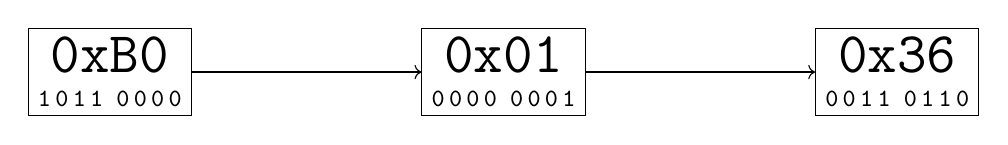
\begin{tikzpicture}
    \texttt{
        \draw (0,0) node[draw, align=center](stsb){
            \huge 0xB0 \\
            \small 1\,0\,1\,1 0\,0\,0\,0
        };
        \draw (5,0) node[draw, align=center](dtb1){
            \huge 0x01 \\
            \small 0\,0\,0\,0 0\,0\,0\,1
        };
        \draw (10,0) node[draw, align=center](dtb2){
            \huge 0x36 \\
            \small 0\,0\,1\,1 0\,1\,1\,0
        };
        \draw[->] (stsb.east) -- (dtb1.west);
        \draw[->] (dtb1.east) -- (dtb2.west);
    }
    \end{tikzpicture}
    \caption{Struktura zprávy \emph{Změna kontroléru} \cite{MIDIspecs}.}
    \label{fig:MIDImsg}
\end{figure}

Z prvního bajtu zprávy z~obr. \ref{fig:MIDImsg} lze dekódovat druh a cílový kanál příkazu. Jedná se o~\emph{Control Change~-- Změna kontroléru} na \emph{kanálu 1}\footnote{$0000_2 \sim \mathrm{kanál\ 1,\ } 0001_2 \sim \mathrm{kanál\ 2}\,\ldots\,1111_2\sim\mathrm{kanál\ 16}$.} Druhý bajt představuje číslo kontroléru (2 -- \emph{Modulation}) a třetí jeho hodnotu (54).

Pro potřeby tohoto semestrálního projektu bude nutné, aby každý přípravek dokázal rozeznat kanál k němu příchozí \acs{MIDI} zprávy, popř. jej pro další přenos pozměnil. \texttt{DATA~BAJTY} budou jen \uv{kopírovány} a nebude do nich nijak zasahováno.

\subsection{Výjimky}\label{chpt:MIDIexcs}
Je třeba alespoň okrajově zmínit výjimečné stavy, které v rámci \acs{MIDI} protokolu mohou nastat. V této fázi semestrální práce nejsou tyto výjimky zatím ošetřeny.

\subsubsection{Running Status}
Pracuje-li \acs{MIDI} vysílač v tomto stavu, neposílá \texttt{STATUS BAJT} v~opakující se zprávě stejného druhu. Přijímač si tedy musí uložit poslední platný \texttt{STATUS BAJT} do paměti, kterou přemaže, obdrží-li zprávu s jiným, novým \texttt{STATUS BAJTEM}. Tento mód výrazně šetří přenesená data, zejména je-li použit při odesílání zprávy \emph{Změna kontroléru} kontinuálních ovladačů \cite{MIDIspecs}.

\subsubsection{Zprávy Real-Time}
Tyto zprávy slouží pro synchronizaci \acs{MIDI} zařízení, které pracují s časovou osou nebo časem obecně. Skládají se pouze z jediného bajtu a mají nejvyšší prioritu. Přijímač by měl být připraven i na to, že je obdrží uprostřed standardní zprávy nebo SysEx zprávy \cite{MIDIspecs}.

\subsubsection{Zprávy SysEx}
SysEx (\emph{System Exlusive}) zprávy se skládají z většího a libovolného počtu bajtů. Jsou víceúčelové a univerzální, používají se například pro posun na časové ose (komplementárně ke zprávám \emph{Real-Time}), \acs{MSC}\footnote{\acl{MSC}} a podobně \cite{MIDIspecs}.

%\section{Softwarová vrstva}
%\begin{circuitikz}
    \draw (0,0) circle(0.5cm) ++ (0,-0.9) node {MIDI OUT};
    \draw (0,0.3) circle(0.07cm) node(midi2){} ++(0.1,0.35) node {\tiny 2};
    \draw (-0.3,0) circle(0.07cm) node(midi3){} ++(-0.35,0) node {\tiny 3};
    \draw (0.3,0) circle(0.07cm) node(midi1){} ++(0.35,0) node {\tiny 1};
    \draw (0.22,0.22) circle(0.07cm) node(midi4){} ++(0.32,0.15) node {\tiny 4};
    \draw (-0.22, 0.22) circle(0.07cm) node(midi5){} ++(-0.32,0.15) node {\tiny 5};
    
    \draw (midi2) -- (0,1.5) to[short,-*] (-1,1.5);
    \draw (midi4) -- (0.7,0.7) -- (0.7,2) -- (-2,2);
    \draw (-4,2) node[left]{\small 5\,V} to[short, o-] ++(0,0) to[R=\footnotesize $220\,\Omega$] (-2,2);
    \draw (midi5) -- (-0.7,0.7) -- (-0.7,1) -- (-2,1);
    \draw (-4,1) to[R=\footnotesize $220\,\Omega$] (-2,1);
    
    \draw[densely dashed] (-1.3,1.5) ellipse (0.3 and 0.9);
    \draw (-1.3,0.6) to[short, -*] ++(0,0) node[ground]{};
    
    \draw (-7,1) to[short,o-] (-6.5,1) to[amp] (-5,1) to[amp, t=\small A] (-4,1);
    \draw (-7,1) node[left]{FROM UART};
    
    
\end{circuitikz}
\chapter{Návrh přípravku}
V~rámci semestrální práce byl vytvořen prototyp zařízení na platformě Arduino~UNO, která disponuje čipem ATMEL ATmega 328P. Arduinu sekunduje \linebreak Ethernet~Shield~V1, který je osazen čipem WizNet W5100. 

Přípravek umožňuje výměnu \acs{MIDI} příkazů přes lokální síť, využívá první čtyři vrstvy ISO/OSI modelu. Zároveň poskytuje pokročilé možnosti směrování jednotlivých \acs{MIDI} kanálů.

\section{Hardware}\label{chpt:Schema}
\begin{figure}[h]
    \centering
    \begin{circuitikz}[]
    \draw (0,0) circle(0.5cm) ++ (0,-0.9) node {MIDI IN};
    \draw (0,0.3) circle(0.07cm) node(m1p2){} ++(0,0.35) node {\tiny 2};
    \draw (-0.3,0) circle(0.07cm) node(m1p3){} ++(-0.35,0) node {\tiny 3};
    \draw (0.3,0) circle(0.07cm) node(m1p1){} ++(0.35,0) node {\tiny 1};
    \draw (0.22,0.22) circle(0.07cm) node(m1p4){} ++(0.32,0.15) node {\tiny 4};
    \draw (-0.22, 0.22) circle(0.07cm) node(m1p5){} ++(-0.32,0.15) node {\tiny 5};
    
    \draw (9,0) circle(0.5cm) ++ (0,-0.9) node {MIDI OUT};
    \draw (9,0.3) circle(0.07cm) node(m2p2){} ++(0.1,0.35) node {\tiny 2};
    \draw (8.7,0) circle(0.07cm) node(m23){} ++(-0.35,0) node {\tiny 3};
    \draw (9.3,0) circle(0.07cm) node(m2p1){} ++(0.35,0) node {\tiny 1};
    \draw (9.22,0.22) circle(0.07cm) node(m2p4){} ++(0.32,0.15) node {\tiny 4};
    \draw (8.78, 0.22) circle(0.07cm) node(m2p5){} ++(-0.32,0.15) node {\tiny 5};
    
    \ctikzset{resistors/scale=0.7}
    \ctikzset{diodes/scale=0.5}
    
    \draw (m1p5) -- (-0.7,0.7) -- (-0.7,4) -- (3,4) to[short, *-] ++(0,0) to[D*] ++(down: 1) to[short, -*] ++(0,0); 
    \draw (m1p4) -- (0.7,0.7) -- (0.7,3) -- (1,3) to[R, l= \footnotesize $R_1$] ++(right: 2);

    \draw (5,3.5) node[dipchip, 
        num pins = 8](OptoIsol){\footnotesize 6N138};

    \draw (3,4) -| (OptoIsol.pin 2);
    \draw (3,3) -| (OptoIsol.pin 3);
    
    \draw (9.1, 3.4) node[dipchip,
        num pins = 10,
        external pins width = 0,
        fill=white,
        hide numbers,
        no topmark]{};
    \draw (9,3.5) node[dipchip,
        num pins = 10,
        external pins width = 0,
        fill=white,
        align=center,
        hide numbers, no topmark](Arduino){\footnotesize{Arduino}\\\footnotesize{WizNet}};
    
    \draw (Arduino.north) node[below]{\tiny 5\,V};
    \coordinate (h1) at (7.3,3.5);
    \draw (Arduino.north) -- ++(up: 0.5) coordinate (h2);
    \draw (h2) to[short, -*] (h2 -| h1) coordinate (middle_top);
    \draw (OptoIsol.pin 8) coordinate (h3) -- (h3 |- h2) -- (middle_top);
    \draw (OptoIsol.pin 6) coordinate (hp6) to[short,-*] (hp6 -| middle_top);
    \draw (middle_top) to[R, l=\footnotesize $R_2$] (middle_top |- hp6);
    \draw (Arduino.pin 5) node[right]{\tiny 4} coordinate (ArP6) -| (middle_top |- hp6);

    \coordinate (h9) at (6.6,3.5);
    \draw (Arduino.south) node[above]{\tiny GND} -- ++(down: 0.5) coordinate (ArPG) -- (ArPG -| OptoIsol.pin 5) -- (OptoIsol.pin 5);
    
    \draw (OptoIsol.pin 7) -- (OptoIsol.pin 7 -| h9) -- (h9 |- OptoIsol.pin 6) to[R,l=\footnotesize$R_3$,-*] (h9 |- ArPG); 

    \draw (m2p4) -- (9.7,0.7) -- ++(right: 0.7) coordinate (h10);
    \draw (h2) to[short,*-] (h2 -| h10) to[R, l=\footnotesize$R_4$] (h10);

    \draw (m2p2) -- ++(up: 0.8) coordinate (m2p2up) -- (m2p2up -| Arduino.south) to[short,-*] (Arduino.south |- ArPG);
    
    \draw (m2p5) -- (8.3,0.7) -- ++(left: 0.6) coordinate(h11) -- (h11 |- Arduino.pin 4) -- (Arduino.pin 4) node[right]{\tiny 5};
    %\draw (OptoIsol.pin 8) -- (h1 |- h2);
    
    

\end{circuitikz}



    \begin{tabular}{l c l c}
        \small
        $R_1$ & $220\,\mathrm{\Omega}$ & $R_2$ & $470\,\mathrm{\Omega}$ \\
        $R_3$ & $10\,\mathrm{k\Omega}$ & $R_4$ & $220\,\mathrm{\Omega}$
    \end{tabular}
    \caption{Schéma prototypu \cite{Indest}} 
    \label{fig:schPrototype}
\end{figure}

Z obr. \ref{fig:schPrototype} je patrné zapojení přípravku. Je využito standardní zapojení \acs{MIDI} vstupu a~výstupu v souladu se schématy na obr.~\ref{fig:schMIDIout} a~\ref{fig:schMIDIin}. Jak již bylo řečeno v kapitole~\ref{chpt:MIDI}, \acs{MIDI} využívá pro komunikaci sériovou linku. V tomto případě je vstupní linka zapojena k~Arduinu na \texttt{pinu~2} a výstupní k~\texttt{pinu~3}\footnote{Arduino umožňuje softwarové přepnutí \texttt{pinů} z režimu výstupu na režim vstup a naopak.}. 

Ve schématu na obr.~\ref{fig:schPrototype} je pro zjednodušení značka \uv{Arduino} chápána jako \uv{Arduino\,+\,Wiznet Shield}.

Přípravek je v~této fázi vývoje napájen skrz \acs{USB} sběrnici Arduina napětím 5\,\unit{V}. 

%...%

\section{Software}
Software přípravku byl vyvíjen za účelem maximalizace variability směřování \acs{MIDI} příkazů. Na funkční rovině je inspirován systémem \emph{Dante}, který se používá pro přenos zvukového signálu přes počítačovou síť. \emph{Dante} umožňuje pokročilé směřování signálů napříč síťovými zařízeními, ovládané pomocí přehledné matice na kontrolním PC. Do této fáze by měl být vyvinut i systém \acs{MoE}\footnote{\acl{MoE}}.
%Pro spolehlivou komunikaci mezi zařízeními bylo třeba vyvinout protokol, který bude zapouzdřovat a směřovat samotné \acs{MIDI} zprávy. S tímto cílem byl implementován protokol \acs{MoE}\footnote{\acl{MoE}}. 
\subsection{Logická vrstva}

Jedna \acs{MoE} zpráva obsahuje \emph{čtyři bajty}. První bajt určuje 






\chapter{Průběh komunikace}
V~této kapitole bude popsán průběh připojení přípravku k síti, automatické rozpoznání a zacházení s přijatými \acs{MIDI} a UDP zprávami.

\section{Připojení k lokální síti}
Každému přípravku byla do prvních šesti bajtů \texttt{EEPROM} paměti uložena unikátní MAC adresa. Při zapnutí a následné inicializaci je adresa načtena a přiřazena. Nejprve proběhne pokus o získání IP adresy pomocí DHCP serveru sítě. V případě neúspěchu použije přípravek uživatelem napevno nastavenou IP adresu. 

Díky knihovně \texttt{EthernetUdp.h} jsou výše zmíněné operace otázkou pouze několika málo řádků:
\lstset{
    frame=single,
    keywordstyle=\color{blue},
    commentstyle=\color{olive},
    basicstyle=\ttfamily\small
    }
\begin{lstlisting}
if (Ethernet.begin())
{
    //DHCP server zdárně přidělil zařízení IP adresu
    Serial.println(Ethernet.localIP());
}
else
{
    Ethernet.begin(_myMac, _userIP);
    //Přidělení IP adresy napevno
    Serial.println(Ethernet.localIP());
}
\end{lstlisting}


\newcommand{\bytes}[4]{
    \begin{center}
        \large{\texttt{0x#1, 0x#2, 0x#3, 0x#4}}
    \end{center}
}



\section{Upozornění na vlastní přítomnost}
Ihned po zdárném připojení k lokální síti je vyslána zpráva  \texttt{beacon}, jejíž účel je upozornit všechna zařízení v lokální síti na vlastní přítomnost. Zpráva se skládá ze čtyř bajtů:
\bytes{FF}{FF}{FF}{FF}
a je poslána na broadcast adresu sítě.

\begin{lstlisting}
_broadcastIP = Ethernet.localIP();
_broadcastIP[3] = 255;
EthernetUdp eUDP;
eUDP.begin(MOE_PORT);
eUDP.beginPacket(_broadcastIP, MOE_PORT);
eUDP.write(_beacon, sizeof(_beacon));
eUDP.endPacket();
\end{lstlisting}

\section{Rozpoznání zařízení na síti}
V případě přijetí zprávy \texttt{beacon} je rozpoznána IP adresa odesílatele a vytvořen nový záznam do databáze spojení \texttt{sub\-scrip\-tions}. V této fázi projektu přípravek napevno přiřazuje kanál 1  lokální příchozí \acs{MIDI} sběrnice kanálu 1 výstupní \acs{MIDI} sběrnice cílového zařízení. V další fázi bude operace přiřazení uskutečňována pravděpodobně přes kontrolní SW na PC připojeného do též sítě.

\begin{lstlisting}
switch(_incomingUDP[0])
{
    //...
    case 0xFF:
        addSubscription(1, eUDP.remoteIP()[3], 1);
    break;
    //...
}
\end{lstlisting}

\section{Přijetí \acs{MIDI} zprávy}\label{chpt:PrijMIDI}
Při přijímání \acs{MIDI} zpráv je nejdříve třeba rozlišit, jedná-li se o zprávou dvoubajtovou, nebo tříbajtovou. Toto lze vyřešit jednoduchým větvením \texttt{switch}. V dalším kroku je nutné dekódovat kanál \acs{MIDI} zprávy z \texttt{DATA BAJTU}~-- tuto \uv{extrakci} lze vyřešit pomocí bitového maskování. Takto získaný bajt je pak porovnáván s prvním nibblem bajtu \texttt{srcdstChannel} každého záznamu databáze \texttt{sub\-scrip\-tions}. Dojde-li ke shodě, začíná konstrukce odchozí zprávy podle dalších informací v odpovídajícím záznamu databáze spojení. Výpis kódu je k dispozici jako příloha \ref{code:handleMIDI}

\section{Přijetí UDP zprávy}
Díky architektuře odesílané zprávy (viz podkapitolu \ref{chpt:PrijMIDI}) je veškeré směrování dokončeno již na straně odesílatele. Přijímač může obdrženou zprávu tedy rovnou poslat do \acs{MIDI} výstupu.



%Nyní je procházena databáze připojení \texttt{sub\-scrip\-tions} a porovnáván první nibble bajtu \texttt{srcdstChannel} každého záznamu s 


%%% Vložení souboru 'text/reseni' s popisem řešení práce
% (rozdělte na více souborů či kapitol, pokud je vhodné)
\chapter{Teoretická část studentské práce}

Teoretické zázemí studentské práce vhodně rozdělené do částí.

(Struktura navržená v~této šabloně je nejhrubší možná, po konzultaci s~vedoucím je vhodné zvolit přiléhavější.)


%%% Vložení souboru 'text/vysledky' s popisem vysledků práce
% (rozdělte na více souborů či kapitol, pokud je vhodné)
\chapter{Výsledky studentské práce}

Praktická část a výsledky studentské práce vhodně rozdělené do částí.

\section{Programové řešení}
Lorem ipsum dolor sit amet, consectetuer adipiscing elit. Nulla pulvinar eleifend sem. Integer in sapien. Etiam sapien elit, consequat eget, tristique non, venenatis quis, ante. In laoreet, magna id viverra tincidunt, sem odio bibendum justo, vel imperdiet sapien wisi sed libero. Phasellus enim erat, vestibulum vel, aliquam a, posuere eu, velit. Aliquam erat volutpat. Nullam faucibus mi quis velit \cite{sr02/2009}.

\section{Výsledky měření}
Fusce tellus odio, dapibus id fermentum quis, suscipit id erat. Fusce tellus. Morbi scelerisque luctus velit. In laoreet, magna id viverra tincidunt, sem odio bibendum justo, vel imperdiet sapien wisi sed libero. Quisque porta. Fusce suscipit libero eget elit. Nulla non lectus sed nisl molestie malesuada. Phasellus faucibus molestie nisl. Integer vulputate sem a nibh rutrum consequat. Proin mattis lacinia justo. Phasellus et lorem id felis nonummy placerat. Etiam ligula pede, sagittis quis, interdum ultricies, scelerisque eu. Cras elementum. Aenean placerat. Donec ipsum massa, ullamcorper in, auctor et, scelerisque sed, est. Aliquam ante. Integer imperdiet lectus quis justo. Vivamus ac leo pretium faucibus. Nullam faucibus mi quis velit.

\subsection{Etiam quis quam}
Neque porro quisquam est, qui dolorem ipsum quia dolor sit amet, consectetur, adipisci velit, sed quia non numquam eius modi tempora incidunt ut labore et dolore magnam aliquam quaerat voluptatem. Aliquam erat volutpat. Lorem ipsum dolor sit amet, consectetuer adipiscing elit \cite{sr02/2009,pravidla}. Nunc auctor. Neque porro quisquam est, qui dolorem ipsum quia dolor sit amet, consectetur, adipisci velit, sed quia non numquam eius modi tempora incidunt ut labore et dolore magnam aliquam quaerat voluptatem. Maecenas lorem. Maecenas libero. In laoreet, magna id viverra tincidunt, sem odio bibendum justo, vel imperdiet sapien wisi sed libero. Nullam rhoncus aliquam metus.

\subsubsection{Integer rutrum orci vestibulum}
Integer rutrum, orci vestibulum ullamcorper ultricies, lacus quam ultricies odio, vitae placerat pede sem sit amet enim. Ut enim ad minim veniam, quis nostrud exercitation ullamco laboris nisi ut aliquip ex ea commodo consequat. Fusce tellus odio, dapibus id fermentum quis, suscipit id erat. Nullam eget nisl. Nunc auctor. Etiam dui sem, fermentum vitae, sagittis id, malesuada in, quam. Fusce dui leo, imperdiet in, aliquam sit amet, feugiat eu, orci. Curabitur vitae diam non enim vestibulum interdum. Aliquam erat volutpat. Pellentesque sapien. Phasellus enim erat, vestibulum vel, aliquam a, posuere eu, velit.

\subsubsection{Eger rutrum orci westibulum}
Fusce dui leo, imperdiet in, aliquam sit amet, feugiat eu, orci. Maecenas aliquet accumsan leo. Aliquam ornare wisi eu metus. Cum sociis natoque penatibus et magnis dis parturient montes, nascetur ridiculus mus. Aliquam erat volutpat. Donec iaculis gravida nulla. Sed elit dui, pellentesque a, faucibus vel, interdum nec, diam. Temporibus autem quibusdam et aut officiis debitis aut rerum necessitatibus saepe eveniet ut et voluptates repudiandae sint et molestiae non recusandae. Nulla non arcu lacinia neque faucibus fringilla. Phasellus enim erat, vestibulum vel, aliquam a, posuere eu, velit. Praesent vitae arcu tempor neque lacinia pretium
\cite{Walter1999,Svacina1999IEEE,RajmicSysel2002}.

Aliquam erat volutpat. Quisque porta. Integer imperdiet lectus quis justo. Nullam justo enim, consectetuer nec, ullamcorper ac, vestibulum in, elit. Nullam faucibus mi quis velit. Fusce tellus. Fusce consectetuer risus a nunc. Cras pede libero, dapibus nec, pretium sit amet, tempor quis. Morbi imperdiet, mauris ac auctor dictum, nisl ligula egestas nulla, et sollicitudin sem purus in lacus
\cite{CSN_ISO_690-2011,CSN_ISO_7144-1997,CSN_ISO_31-11}.
Mauris elementum mauris vitae tortor. Neque porro quisquam est, qui dolorem ipsum quia dolor sit amet, consectetur, adipisci velit, sed quia non numquam eius modi tempora incidunt ut labore et dolore magnam aliquam quaerat voluptatem. Quisque porta. Integer vulputate sem a nibh rutrum consequat. Nulla pulvinar eleifend sem. Praesent id justo in neque elementum ultrices \cite{BiernatovaSkupa2011:CSNISO690komentar}.

Fusce suscipit libero eget elit. Integer vulputate sem a nibh rutrum consequat. Aliquam erat volutpat. Etiam neque. Nulla turpis magna, cursus sit amet, suscipit a, interdum id, felis. Nullam rhoncus aliquam metus. Etiam dui sem, fermentum vitae, sagittis id, malesuada in, quam. Nunc auctor. Nunc dapibus tortor vel mi dapibus sollicitudin. Praesent in mauris eu tortor porttitor accumsan. Nulla non arcu lacinia neque faucibus fringilla. Nullam lectus justo, vulputate eget mollis sed, tempor sed magna. Maecenas lorem. Aenean placerat. Donec vitae arcu. Maecenas lorem. Donec iaculis gravida nulla. Nulla non lectus sed nisl molestie malesuada.

Duis pulvinar. Nulla est. Duis condimentum augue id magna semper rutrum. Integer pellentesque quam vel velit. Aliquam ante. Nulla quis diam. Proin mattis lacinia justo. Aenean fermentum risus id tortor. Nunc auctor. Nullam justo enim, consectetuer nec, ullamcorper ac, vestibulum in, elit. In dapibus augue non sapien. Etiam bibendum elit eget erat. In sem justo, commodo ut, suscipit at, pharetra vitae, orci. Maecenas libero.

Nulla non lectus sed nisl molestie malesuada. Donec vitae arcu. Aenean fermentum risus id tortor. Praesent in mauris eu tortor porttitor accumsan. Nulla pulvinar eleifend sem. Duis viverra diam non justo. Integer imperdiet lectus quis justo. Pellentesque habitant morbi tristique senectus et netus et malesuada fames ac turpis egestas. In rutrum. Excepteur sint occaecat cupidatat non proident, sunt in culpa qui officia deserunt mollit anim id est laborum. Nulla non lectus sed nisl molestie malesuada. Aliquam erat volutpat. Mauris tincidunt sem sed arcu. Duis bibendum, lectus ut viverra rhoncus, dolor nunc faucibus libero, eget facilisis enim ipsum id lacus. Fusce tellus odio, dapibus id fermentum quis, suscipit id erat. In enim a arcu imperdiet malesuada. Nulla non lectus sed nisl molestie malesuada. Proin mattis lacinia justo.

Aliquam in lorem sit amet leo accumsan lacinia. Cum sociis natoque penatibus et magnis dis parturient montes, nascetur ridiculus mus. Duis sapien nunc, commodo et, interdum suscipit, sollicitudin et, dolor. Suspendisse sagittis ultrices augue. Nullam lectus justo, vulputate eget mollis sed, tempor sed magna. In convallis. Praesent id justo in neque elementum ultrices. Neque porro quisquam est, qui dolorem ipsum quia dolor sit amet, consectetur, adipisci velit, sed quia non numquam eius modi tempora incidunt ut labore et dolore magnam aliquam quaerat voluptatem.

Pellentesque pretium lectus id turpis. Nemo enim ipsam voluptatem quia voluptas sit aspernatur aut odit aut fugit, sed quia consequuntur magni dolores eos qui ratione voluptatem sequi nesciunt. Curabitur ligula sapien, pulvinar a vestibulum quis, facilisis vel sapien. Praesent dapibus. Sed elit dui, pellentesque a, faucibus vel, interdum nec, diam. Duis viverra diam non justo. Duis ante orci, molestie vitae vehicula venenatis, tincidunt ac pede. Phasellus rhoncus. Maecenas fermentum, sem in pharetra pellentesque, velit turpis volutpat ante, in pharetra metus odio a lectus. Proin pede metus, vulputate nec, fermentum fringilla, vehicula vitae, justo. Fusce aliquam vestibulum ipsum. Nullam at arcu a est sollicitudin euismod.

%Aliquam ante. Phasellus faucibus molestie nisl. Etiam ligula pede, sagittis quis, interdum ultricies, scelerisque eu. Morbi leo mi, nonummy eget tristique non, rhoncus non leo. Cum sociis natoque penatibus et magnis dis parturient montes, nascetur ridiculus mus. Morbi scelerisque luctus velit. Curabitur bibendum justo non orci. Donec quis nibh at felis congue commodo. Nullam faucibus mi quis velit. Aenean id metus id velit ullamcorper pulvinar. Pellentesque sapien. Fusce nibh. Vestibulum fermentum tortor id mi. Nullam eget nisl. Praesent vitae arcu tempor neque lacinia pretium. Proin in tellus sit amet nibh dignissim sagittis. Donec quis nibh at felis congue commodo.
%
%Nam quis nulla. Proin in tellus sit amet nibh dignissim sagittis. Nullam dapibus fermentum ipsum. Curabitur ligula sapien, pulvinar a vestibulum quis, facilisis vel sapien. Nam libero tempore, cum soluta nobis est eligendi optio cumque nihil impedit quo minus id quod maxime placeat facere possimus, omnis voluptas assumenda est, omnis dolor repellendus. Vivamus ac leo pretium faucibus. Nunc tincidunt ante vitae massa. Maecenas sollicitudin. Ut tempus purus at lorem. Nullam lectus justo, vulputate eget mollis sed, tempor sed magna. Fusce consectetuer risus a nunc. Etiam quis quam.
%
%Donec quis nibh at felis congue commodo. Sed vel lectus. Donec odio tempus molestie, porttitor ut, iaculis quis, sem. Nullam feugiat, turpis at pulvinar vulputate, erat libero tristique tellus, nec bibendum odio risus sit amet ante. Sed elit dui, pellentesque a, faucibus vel, interdum nec, diam. Cras elementum. Sed vel lectus. Donec odio tempus molestie, porttitor ut, iaculis quis, sem. Etiam neque. Integer tempor. Vivamus porttitor turpis ac leo. Nulla non arcu lacinia neque faucibus fringilla.
%
%Etiam posuere lacus quis dolor. Nemo enim ipsam voluptatem quia voluptas sit aspernatur aut odit aut fugit, sed quia consequuntur magni dolores eos qui ratione voluptatem sequi nesciunt. Nullam faucibus mi quis velit. Cum sociis natoque penatibus et magnis dis parturient montes, nascetur ridiculus mus. Phasellus faucibus molestie nisl. Maecenas ipsum velit, consectetuer eu lobortis ut, dictum at dui. Maecenas aliquet accumsan leo. Pellentesque ipsum. Donec vitae arcu. Suspendisse nisl. Morbi imperdiet, mauris ac auctor dictum, nisl ligula egestas nulla, et sollicitudin sem purus in lacus. Pellentesque ipsum. Ut enim ad minima veniam, quis nostrum exercitationem ullam corporis suscipit laboriosam, nisi ut aliquid ex ea commodi consequatur? Nam libero tempore, cum soluta nobis est eligendi optio cumque nihil impedit quo minus id quod maxime placeat facere possimus, omnis voluptas assumenda est, omnis dolor repellendus.


%%% Vložení souboru 'text/zaver' se závěrem
\chapter*{Závěr}
\phantomsection
\addcontentsline{toc}{chapter}{Závěr}

Výstupem této semestrální práce je funkční přípravek, který disponuje ethernetovým a vstupním i výstupním \acs{MIDI} rozhraním. Přípravek se automaticky připojí do počítačové sítě a dále funguje již autonomně. Dokáže přijmout \acs{MIDI} zprávu, přeformátovat ji v souladu s daným záznamem databáze spojení a s využitím \acs{UDP} protokolu poslat správnému příjemci. Databáze spojení je taktéž editovatelná na dálku pomocí programu \emph{MoE Matrix Editor}. 

Stále však existuje mnoho prostoru pro optimalizaci. Pokud přípravek obdrží více než dvě \acs{MIDI} zprávy těsně za sebou, přestane přijímat jakékoliv další bajty a jeho funkčnost je do restartu přerušena. Absence implementace ošetření výjimek (dle kapitoly \ref{chpt:MIDIexcs}) zase prozatím brání využití přípravků tam, kde je příjem zpráv v módu Running Status nebo SysEx standardem.

Jako uspokojivé lze však vnímat dosažené hodnoty latence mezi přijetím \acs{MIDI} zprávy na sériové sběrnici jednoho zařízení a odeslání též zprávy na sériovou sběrnici zařízení druhého. Komunikace mezi samotnými zařízeními samozřejmě probíhala prostřednictvím počítačové sítě. Dle přílohy \ref{fig:Latency1} vykazuje dolní hranice celkové latence \acs{MoE} řešení $2{,}18\,\unit{ms}$ v případě jediného záznamu v databázi spojení. S každým dalším záznamem pak latence přirozeně roste. Maximální naměřená hodnota latence (mezi první přijatou a poslední odeslanou zprávou) pak dosahovala $20{,}92\,\unit{ms}$. Při živé hudební produkci s využitím \acs{MIDI} klávesového nástroje by neměla celková latence přesáhnout 5\,ms. S touto premisou lze prohlásit, že \acs{MoE} řešení by mohlo být za určitých podmínek použitelné i pro časově náročnější podmínky.

%%% Vložení souboru 'text/literatura' se seznamem zdrojů
% Pro sazbu seznamu literatury použijte jednu z následujících možností

%%%%%%%%%%%%%%%%%%%%%%%%%%%%%%%%%%%%%%%%%%%%%%%%%%%%%%%%%%%%%%%%%%%%%%%%%
%1) Seznam citací definovaný přímo pomocí prostředí literatura / thebibliography

\begin{thebibliography}{99}

    \bibitem{Indest}
    GHASSAEI, Amanda. \emph{Send and Receive MIDI With Arduino}\/ [online]. [cit.\,1.\,12.\,2020]. Dostupné z~URL: <\url{https://www.instructables.com/Send-and-Receive-MIDI-with-Arduino/}>.

    \bibitem{vkMIDI}
    GUÉRIN, Robert. \emph{Velká kniha MIDI: standardy, hardware, software}. Brno: Computer Press, 2004. 328~s. ISBN 80-722-6985-2.

    \bibitem{MIDIspecs}
    MIDI MANUFACTURERS ASSOCIATION, The. \emph{MIDI 1.0 Detailed Specification.} Document Version 4.2.1. Los Angeles, CA: MMA, 1996. 58~s. Dostupné také z:~<\url{https://www.midi.org/specifications/m1-v4-2-1-midi-1-0-detailed-specification-96-1-4/download}>.

    \bibitem{MIDIupd}
    MMA TECHNICAL STANDARDS BOARD/AMEI MIDI COMMITTEE. \emph{MIDI 1.0 Electrical Specification Update.} 2014. s.\,1--3. Dostupné také z:\\<\url{https://www.midi.org/downloads?task=callelement&format=raw&item_id=100&element=f85c494b-2b32-4109-b8c1-083cca2b7db6&method=download}>.

    \bibitem{UDPpaper}
    MNEIMNEH, Saad. \emph{Computer Networks UDP and TCP}. Hunter College of CUNY. New York. 2008. Dostupné také z:~<\url{http://www.cs.hunter.cuny.edu/~saad/courses/networks/notes/note7.pdf}>.




	



%
%    \bibitem{sr02/2009}
%		VUT v~Brně:
%    \emph{Úprava, odevzdávání a zveřejňování vysokoškolských %kva\-li\-fi\-kač\-ních prací na VUT v~Brně}\/ [online].
%		Směrnice rektora č.\,2/2009.
%		Brno: 2009, po\-sled\-ní aktualizace 24.\,3.\,2009 [cit.\,23.\,%10.\,2015].
%    Dostupné z~URL:\\
%    <\url{https://www.vutbr.cz/uredni-deska/vnitrni-predpisy-a-dokumenty/%smernice-rektora-f34920/}>.
%
%\bibitem{CSN_ISO_690-2011}
%    \emph{ČSN ISO 690 (01 0197) Informace a dokumentace -- Pravidla pro %bibliografické odkazy a citace informačních zdrojů.}
%    40 stran. Praha: Český normalizační institut, 2011.
%
%\bibitem{CSN_ISO_7144-1997}
%    \emph{ČSN ISO 7144 (010161) Dokumentace -- Formální úprava disertací %a podobných dokumentů.}
%    24 stran. Praha: Český normalizační institut, 1997.
%
%\bibitem{CSN_ISO_31-11}
%    \emph{ČSN ISO 31-11 Veličiny a jednotky -- část 11: Matematické znaky %a značky používané ve fyzikálních vědách a v~technice.}
%    Praha: Český normalizační institut, 1999.
%
%\bibitem{BiernatovaSkupa2011:CSNISO690komentar}
%    BIERNÁTOVÁ, O., SKŮPA, J.:
%    \emph{Bibliografické odkazy a citace dokumentů dle ČSN ISO 690 (01 %0197) platné od 1.\,dubna 2011}\/ [online].
%    2011, poslední aktualizace 2.\,9.\,2011 [cit. 19.\,10.\,2011].
%    Dostupné z~URL:
%    \(<\)\url{http://www.citace.com/CSN-ISO-690.pdf}\(>\)
%%    \(<\)\href{http://www.boldis.cz/citace/citace.html}{http://%www.boldis.cz/citace/citace.html}\(>\).
%
%\bibitem{pravidla}
%    \emph{Pravidla českého pravopisu}.
%    Zpracoval kolektiv autorů. 1.\ vydání.
%    Olomouc: FIN PUB\-LISH\-ING, 1998. 575 s. ISBN 80-86002-40-3.
%
%\bibitem{Walter1999}
%	WALTER, G.\,G.; SHEN, X.
%	\emph{Wavelets and Other Orthogonal Systems}.
%	2. vyd. Boca Raton: Chapman\,\&\,Hall/CRC, 2000. 392~s. ISBN %1-58488-227-1
%
%\bibitem{Svacina1999IEEE}
%	SVAČINA, J.
%	Dispersion Characteristics of Multilayered Slotlines -- a Simple %Approach.
%	\emph{IEEE Transactions on Microwave Theory and Techniques},
%	1999, vol.\,47, no.\,9, s.\,1826--1829. ISSN 0018-9480.
%
%\bibitem{RajmicSysel2002}
%    RAJMIC, P.; SYSEL, P.
%    Wavelet Spectrum Thresholding Rules.
%    In \emph{Proceedings of the International Conference Research in %Telecommunication Technology},
%    Žilina: Žilina University, 2002. s.\,60--63. ISBN 80-7100-991-1.
%
\end{thebibliography}


%%%%%%%%%%%%%%%%%%%%%%%%%%%%%%%%%%%%%%%%%%%%%%%%%%%%%%%%%%%%%%%%%%%%%%%%%
%%2) Seznam citací pomocí BibTeXu
%% Při použití je nutné v TeXnicCenter ve výstupním profilu aktivovat spouštění BibTeXu po překladu.
%% Definice stylu seznamu
%\bibliographystyle{unsrturl}
%% Pro českou sazbu lze použít styl czechiso.bst ze stránek
%% http://www.fit.vutbr.cz/~martinek/latex/czechiso.tar.gz
%%\bibliographystyle{czechiso}
%% Vložení souboru se seznamem citací
%\bibliography{text/literatura}
%
%% Následující příkaz je pouze pro ukázku sazby literatury při použití BibTeXu.
%% Způsobí citaci všech zdrojů v souboru odkazy.bib, i když nejsou citovány v textu.
%\nocite{*}

%%% Vložení souboru 'text/zkratky' se seznam použitých symbolů, veličin a zkratek
\cleardoublepage
\chapter*{\listofabbrevname}
\phantomsection
\addcontentsline{toc}{chapter}{\listofabbrevname}

\begin{acronym}[KolikMista]
    \acro{DAW}
    {Digital Audio Workstation -- digitální pracovní stanice pro náběr a úpravu vícestopého záznamu.}
    \acro{LED}
    {Light-Emiting Diode -- dioda, která vyzařuje viditelné světlo.}
    \acro{MIDI}
    {Musical Instrument Digital Interface -- digitální rozhraní hudebního nástroje}
    \acro{MoE}
    {\acs{MIDI} over Ethernet~-- \acs{MIDI} po Ethernetu}
    \acro{MSb}
    {Most Significant bit -- nejvýznamnější bit (většinou v bajtu).}
    \acro{MSC}
    {\acs{MIDI} Show Control -- subprotokol pro ovládání scénické techniky, zejména pomocí příkazů GO, STOP, popř. RESUME. \cite{MIDIspecs}}
    \acro{RF}
    {Radio Frequency}
    \acro{UART}
    {Universal Asynchronous Receiver/Transmitter -- univerzální asynchronní přijímač/vysílač.}
    \acro{UDP}
    {User Datagram Protocol~-- jednoduchý síťový protokol, který umožňuje výměnu zpráv \uv{host-to-host} \cite{UDPpaper}.}
    \acro{USB}
    {Universal Serial Bus -- univerzální sériová sběrnice pro komunikace s periferními zařízeními.}







%	\acro{zkTemp}		% název
%		[Šířka levého sloupce Seznamu symbolů, veličin a zkratek]	%							% zkratka
%		{je určena šířkou parametru prostředí \texttt{acronym} (viz %řádek~1 výpisu zdrojáku na~str.\,\pageref{lst:zkratky})}
%											% rozvinutí zkratky
%
%	\acro{zkDummy}
%		[KolikMista]
%		{pouze ukázka vyhrazeného místa}
%
%	\acro{DSP}		% název/zkratka
%		{číslicové zpracování signálů -- Digital Signal Processing}
%											% rozvinutí zkratky
%	%%% bsymfvz
%	\acro{symfvz}						% název
%		[\ensuremath{f_\textind{vz}}] % symbol
%		{vzorkovací kmitočet}					% popis
%	%%% esymfvz

\end{acronym}


%%% Začátek příloh
\appendix

%%% Vysázení seznamu příloh
% (vynechejte, pokud máte dvě nebo méně příloh)
\listofappendices

%%% Vložení souboru 'text/prilohy' s přílohami
% Obvykle je přítomen alespoň popis co najdeme na přiloženém médiu
\chapter{\acs{MIDI} STATUS BAJTY}
\begin{table}[h]
    \centering
    \begin{tabular}{|l|l|c|c|}
     \hline
     \multicolumn{2}{|c|}{Název} & Hex. hodnota & Bin. hodnota \\  
     \hline\hline 
     Note-Off & Nota vypnuta & 8n & 1000 nnnn \\
     Note-On & Nota zapnuta & 9n & 1001 nnnn \\
     Poly Key Pressure & Polyfonický tlakový ovladač & An & 1010 nnnn \\
     Control Change & Změna kontroléru & Bn & 1011 nnnn \\
     Program Change & Změna programu & Cn & 1100 nnnn \\
     Channel Pressure & Monofonický tlakový ovladač & Dn & 1101 nnnn \\
     Pitch Bend & Ohyb výšky tónu & En & 1110 nnnn \\
     \hline
\end{tabular}
    \caption{Tabulka \acs{MIDI} \texttt{STATUS BAJTŮ} \cite{MIDIspecs}.}
    \label{tab:MIDIsts}
\end{table}

\chapter{Výpis kódu pro příjem a zpracování \acs{MIDI} zprávy}\label{code:handleMIDI}
\begin{lstlisting}
void handleMIDI()
	{
		int numIncBytes = midiSerial.available();
		if (numIncBytes) 
		{
			switch (numIncBytes)
			{
				//...
				case 3:
					byte data0, data1, data2;
					data0 = midiSerial.read();
					data1 = midiSerial.read();
					data2 = midiSerial.read();
					sendUDP(data0, data1, true, data2);
				break;
				//...
			}
		}
	}
	
	void sendUDP(byte data0, byte data1, bool threeByte, 
				 byte data2)
	{
		byte srcCh = data0 & 0x0F;
		for (byte i = 0; i < MAX_SUBS; i++)
		{
			if (srcCh == (_subscriptions[i].srcdstChannel 
							& 0xF0) >> 4)
			{
				data0 = data0 & 0xF0;
				data0 = data0 | (_subscriptions[i].srcdstChannel 
								& 0x0F);
				IPAddress remoteIP = Ethernet.localIP();
				remoteIP[3] = _subscriptions[i].dstIPnib;
				eUDP.beginPacket(remoteIP, MOE_PORT);
				eUDP.write(0xAA);
				eUDP.write(data0);
				eUDP.write(data1);
				if (threeByte)
					eUDP.write(data2);
				eUDP.endPacket();
			}
		}
	}
	\end{lstlisting}




\chapter{Některé příkazy balíčku \texttt{thesis}}

\section{Příkazy pro sazbu veličin a jednotek}

\begin{table}[!h]
  \caption[Přehled příkazů]{Přehled příkazů pro matematické prostředí }
  \begin{center}
  	\small
	  \begin{tabular}{|c|c|c|c|}
	    \hline
	    Příkaz    						& Příklad 					& Zdroj příkladu  							& Význam  \\
	    \hline\hline
	    \verb|\textind{...}|	& $\beta_\textind{max}$ 	& \verb|$\beta_\textind{max}$|	& textový index \\
	    \hline
	    \verb|\const{...}| 		& $\const{U}_\textind{in}$ 				& \verb|$\const{U}_\textind{in}$|		& konstantní veličina \\
	    \hline
	    \verb|\var{...}| 		& $\var{u}_\textind{in}$ & \verb|$\var{u}_\textind{in}$| & proměnná veličina \\
	    \hline
	    \verb|\complex{...}| 	& $\complex{u}_\textind{in}$ & \verb|$\complex{u}_\textind{in}$| & komplexní veličina \\
	    \hline
	    \verb|\vect{...}| 		& $\vect{y}$ 						& \verb|$\vect{y}$| & vektor \\
	    \hline
	    \verb|\mat{...}| 	& $\mat{Z}$ 						& \verb|$\mat{Z}$| & matice \\
	    \hline
	    \verb|\unit{...}| 		& $\unit{kV}$ 						& \verb|$\unit{kV}$|\quad či\ \, \verb|\unit{kV}| & jednotka \\
	    \hline
	  \end{tabular}
  \end{center}
\end{table}



%\newpage
\section{Příkazy pro sazbu symbolů}

\begin{itemize}
  \item
    \verb|\E|, \verb|\eul| -- sazba Eulerova čísla: $\eul$,
  \item
    \verb|\J|, \verb|\jmag|, \verb|\I|, \verb|\imag| -- sazba imaginární jednotky: $\jmag$, $\imag$,
  \item
    \verb|\dif| -- sazba diferenciálu: $\dif$,
  \item
    \verb|\sinc| -- sazba funkce: $\sinc$,
  \item
    \verb|\mikro| -- sazba symbolu mikro stojatým písmem%
			\footnote{znak pochází z~balíčku \texttt{textcomp}}: $\mikro$,
	\item
		\verb|\uppi| -- sazba symbolu $\uppi$
			(stojaté řecké pí, na rozdíl od \verb|\pi|, což sází $\pi$).
\end{itemize}
%
Všechny symboly jsou určeny pro matematický mód, vyjma \verb|\mikro|, jenž je\\ použitelný rovněž v~textovém módu.
%$\upmikro$


\chapter{Druhá příloha}

\begin{figure}[!h]
  \begin{center}
    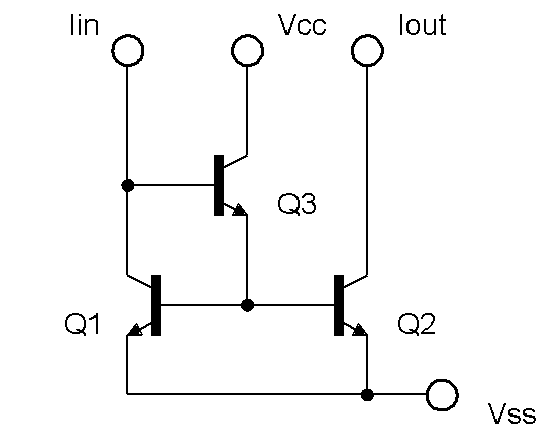
\includegraphics[scale=0.5]{obrazky/ZlepseneWilsonovoZrcadloNPN}
  \end{center}
  \caption[Alenčino zrcadlo]{Zlepšené Wilsonovo proudové zrcadlo.}
\end{figure}

Pro sazbu vektorových obrázků přímo v~\LaTeX{}u je možné doporučit balíček \href{https://www.ctan.org/pkg/pgf}{\texttt{TikZ}}.
Příklady sazby je možné najít na \href{http://www.texample.net/tikz/examples/}{\TeX{}ample}.
Pro vyzkoušení je možné použít programy QTikz nebo TikzEdt.




\chapter{Příklad sazby zdrojových kódů}

\section{Balíček \texttt{listings}}

Pro vysázení zdrojových souborů je možné použít balíček \href{https://www.ctan.org/pkg/listings}{\texttt{listings}}.
Balíček zavádí nové prostředí \texttt{lstlisting} pro sazbu zdrojových kódů, jako například:
%
\begin{lstlisting}[language={[LaTeX]TeX}]
\section{Balíček lstlistings}
Pro vysázení zdrojových souborů je možné použít
	balíček \href{https://www.ctan.org/pkg/listings}%
	{\texttt{listings}}.
Balíček zavádí nové prostředí \texttt{lstlisting} pro
	sazbu zdrojových kódů.
\end{lstlisting}
%
Podporuje množství programovacích jazyků.
Kód k~vysázení může být načítán přímo ze zdrojových souborů.
Umožňuje vkládat čísla řádků nebo vypisovat jen vybrané úseky kódu.
Např.:

\noindent
Zkratky jsou sázeny v~prostředí \texttt{acronym}:
\label{lst:zkratky}
\lstinputlisting[language={[LaTeX]TeX},nolol,numbers=left, firstnumber=6, firstline=6,lastline=6]{text/zkratky.tex}
%
Šířka textu volitelného parametru \verb|KolikMista| udává šířku prvního sloupce se zkratkami.
Proto by měla být zadávána nejdelší zkratka nebo symbol.
Příklad definice zkratky \acs{symfvz} je na výpisu \ref{lst:symfvz}.

\shorthandoff{-}
\lstinputlisting[language={[LaTeX]TeX},frame=single,caption={Ukázka sazby zkratek},label=lst:symfvz,numbers=left,linerange={bsymfvz-\%\%\%\ esymfvz},includerangemarker=false]{text/zkratky.tex}
\shorthandon{-}

\noindent
Ukončení seznamu je provedeno ukončením prostředí:
\lstinputlisting[language={[LaTeX]TeX},nolol,numbers=left,firstnumber=26,linerange=26]{text/zkratky.tex}

\vspace{\fill}

\noindent
{\bf Poznámka k~výpisům s~použitím volby jazyka \verb|czech| nebo \verb|slovak|:}\newline
Pokud Váš zdrojový kód obsahuje znak spojovníku \verb|-|, pak překlad může skončit chybou.
Ta je způsobená tím, že znak \verb|-| je v~českém nebo slovenském nastavení balíčku \verb|babel| tzv.\ aktivním znakem.
Přepněte znak \verb|-| na neaktivní příkazem \verb|\shorthandoff{-}| těsně před výpisem a hned za ním jej vraťte na aktivní příkazem \verb|\shorthandon{-}|.
Podobně jako to je ukázáno ve zdrojovém kódu šablony.


\clearpage

%\section{Výpis kódu prostředí Matlab}
Na výpisu \ref{lst:priklad.vypis.kodu.Matlab} naleznete příklad kódu pro Matlab, na výpisu \ref{lst:priklad.vypis.kodu.C} zase pro jazyk~C.

\lstnewenvironment{matlab}[1][]{%
\iflanguage{czech}{\shorthandoff{-}}{}%
\iflanguage{slovak}{\shorthandoff{-}}{}%
\lstset{language=Matlab,numbers=left,#1}%
}{%
\iflanguage{slovak}{\shorthandon{-}}{}%
\iflanguage{czech}{\shorthandon{-}}{}%
}

\begin{matlab}[frame=single,float=htbp,caption={Příklad Schur-Cohnova testu stability v~prostředí Matlab.},label=lst:priklad.vypis.kodu.Matlab,numberstyle=\scriptsize, numbersep=7pt]
%% Priklad testovani stability filtru

% koeficienty polynomu ve jmenovateli
a = [ 5, 11.2, 5.44, -0.384, -2.3552, -1.2288];
disp( 'Polynom:'); disp(poly2str( a, 'z'))

disp('Kontrola pomoci korenu polynomu:');
zx = roots( a);
if( all( abs( zx) < 1))
    disp('System je stabilni')
else
    disp('System je nestabilni nebo na mezi stability');
end

disp(' '); disp('Kontrola pomoci Schur-Cohn:');
ma = zeros( length(a)-1,length(a));
ma(1,:) = a/a(1);
for( k = 1:length(a)-2)
    aa = ma(k,1:end-k+1);
    bb = fliplr( aa);
    ma(k+1,1:end-k+1) = (aa-aa(end)*bb)/(1-aa(end)^2);
end

if( all( abs( diag( ma.'))))
    disp('System je stabilni')
else
    disp('System je nestabilni nebo na mezi stability');
end
\end{matlab}

\noindent
\begin{minipage}{\linewidth}


%\section{Výpis kódu jazyka C}

\begin{lstlisting}[frame=single,numbers=right,caption={Příklad implementace první kanonické formy v~jazyce C.},label=lst:priklad.vypis.kodu.C,basicstyle=\ttfamily\small, keywordstyle=\color{black}\bfseries\underbar,]
// první kanonická forma
short fxdf2t( short coef[][5], short sample)
{
	static int v1[SECTIONS] = {0,0},v2[SECTIONS] = {0,0};
	int x, y, accu;
	short k;

	x = sample;
	for( k = 0; k < SECTIONS; k++){
		accu = v1[k] >> 1;
		y = _sadd( accu, _smpy( coef[k][0], x));
		y = _sshl(y, 1) >> 16;

		accu = v2[k] >> 1;
		accu = _sadd( accu, _smpy( coef[k][1], x));
		accu = _sadd( accu, _smpy( coef[k][2], y));
		v1[k] = _sshl( accu, 1);

		accu = _smpy( coef[k][3], x);
		accu = _sadd( accu, _smpy( coef[k][4], y));
		v2[k] = _sshl( accu, 1);

		x = y;
	}
	return( y);
}
\end{lstlisting}
\end{minipage}







\chapter{Obsah přiloženého CD}
Nezapomeňte uvést, co čtenář najde na přiloženém médiu.
Je vhodné okomentovat obsah každého adresáře, specifikovat, který soubor obsahuje důležitá nastavení, který soubor je určen ke spuštění atd.
Také je dobře napsat, v~jaké verzi software byl kód testován (např.\ Matlab 2010b).

Pokud je souborů hodně a jsou organizovány ve více složkách,  je možné pro výpis adresářové struktury použít balíček \href{https://www.ctan.org/pkg/dirtree}{\texttt{dirtree}}.

{\small
%
\dirtree{%.
.1 /\DTcomment{kořenový adresář přiloženého CD}.
.2 logo\DTcomment{loga školy a fakulty}.
.3 BUT\_abbreviation\_color\_PANTONE\_EN.pdf.
.3 BUT\_color\_PANTONE\_EN.pdf.
.3 FEEC\_abbreviation\_color\_PANTONE\_EN.pdf.
.3 FEKT\_zkratka\_barevne\_PANTONE\_CZ.pdf.
.3 UTKO\_color\_PANTONE\_CZ.pdf.
.3 UTKO\_color\_PANTONE\_EN.pdf.
.3 VUT\_barevne\_PANTONE\_CZ.pdf.
.3 VUT\_symbol\_barevne\_PANTONE\_CZ.pdf.
.3 VUT\_zkratka\_barevne\_PANTONE\_CZ.pdf.
.2 obrazky\DTcomment{ostatní obrázky}.
.3 soucastky.png.
.3 spoje.png.
.3 ZlepseneWilsonovoZrcadloNPN.png.
.3 ZlepseneWilsonovoZrcadloPNP.png.
.2 pdf\DTcomment{pdf stránky generované informačním systémem}.
.3 student-desky.pdf.
.3 student-titulka.pdf.
.3 student-zadani.pdf.
.2 text\DTcomment{zdrojové textové soubory}.
.3 literatura.tex.
.3 prilohy.tex.
.3 reseni.tex.
.3 uvod.tex.
.3 vysledky.tex.
.3 zaver.tex.
.3 zkratky.tex.
%.2 navod-sablona\_FEKT.pdf\DTcomment{návod na používání šablony}.
.2 sablona-obhaj.tex\DTcomment{hlavní soubor pro sazbu prezentace k~obhajobě}.
%.2 readme.txt\DTcomment{soubor s~popisem obsahu CD}.
.2 sablona-prace.tex\DTcomment{hlavní soubor pro sazbu kvalifikační práce}.
.2 thesis.sty\DTcomment{balíček pro sazbu kvalifikačních prací}.
}
}


\end{document}